\chapter{Related works}
\label{cap:cap03}

The work in \cite{Rethinking} presents an implementation of a BRAS/BNG using an alternative framework called Click. It comes with hundred of simple elements. Moreover, it uses tiny virtual machines that can boot quickly and have a small memory footprint,  it lends itself to a good platform for NFV, and the results reported focus on the overall performance of a number of session establishment rate and memory consumption when establishing sessions instead of the impact of design decisions on performance.\\

The work in \cite{Masutani} describes a BNG implementation but focuses on a vendor-neutral architecture suitable for standardization. They present the requirements and a basic design of
a flexible and elastic network service infrastructure with NFV and SDN/OpenFlow. Our work differs in that adds other features such as multi-architecture target using MACSAD tool and P4 language in order to add more flexibility and application performance.\\

The work in \cite{Nemeth} exposes the performance implications related bandwidth constraints, Virtual Network Function (VNF) placement during service deployment.  They illustrate this with a “proof of concept” implementation of a Broadband Remote Access Service (BRAS)/Border Network Gateway (BNG) using Data Plane Development Kit (DPDK) \cite{dpdk}. The performance focuses on the QoS function, the most resource demanding function of their prototype, and the impact of core layout and memory usage on performance.\\


In order to turn more flexible \cite{Pongracz} describes the implementation of a router using DPDK. He reported forwarding rates between 5.26 Gbps and 9.6 Gbps for packet sizes of 64B and 512B, respectively, with one OpenFlow 1.3 implementation as the primary model of SDN data plane. Our routing functions are substantially similar to theirs, and both implementations use DPDK framework to add functionalities to the network device.\\


The work in \cite{Hwang} describes the design of software router, with some network functionalities such as Layer 3 forwarding, a firewall that resides in distinct VMs on the NetVM platform obtaining throughputs up to 10 Gbps. Rather of running into hardware limitations such as NIC, their implementation is limited by the available processing capacity.\\

The work in \cite{Woesner} shows a BRAS / BNG demo scenario to migrate PPPoE / PPP-based Internet access to a plain IPoE network functionalities and develop BNG and BRAS prototypes into an orchestration framework triggered by an SDN and NFV control. Unlike our proposed work their implementation doesn't have results of the implementation as such as worst and best cases of throughput neither functionalities validation, application performance and memory usage.\\

In \cite{Rahimi} they evaluated the impact of certain parameters and settings in a software switch called Lagopus on which were implemented L2 and L3 network layer functionalities using Intel’s Data Plane Development Kit (DPDK) and OpenFlow.\\
This work focused on application performance using a software called “pktgen” achieving  maximum throughput of 9.8 Gbps when the packet size was 1500B and 100K OpenFlow entry tables in other hand they studied packet drop rates and presented the impact of parallelization on switch performance, which includes both packet forwarding rate and packet drop rate, at high loads in a configuration with high link rates it demonstrates the importance of receive-thread packet classification for load balancing and to send delay-sensitive flows to a different worker thread from high-throughput flows.

Main related projects around BNG software switch implementations and data plane support mentioned above are summarized in Table \ref{table:related_w}:

\begin{table}[H]
	\begin{tabular}{ >{\arraybackslash}m{20cm}}
		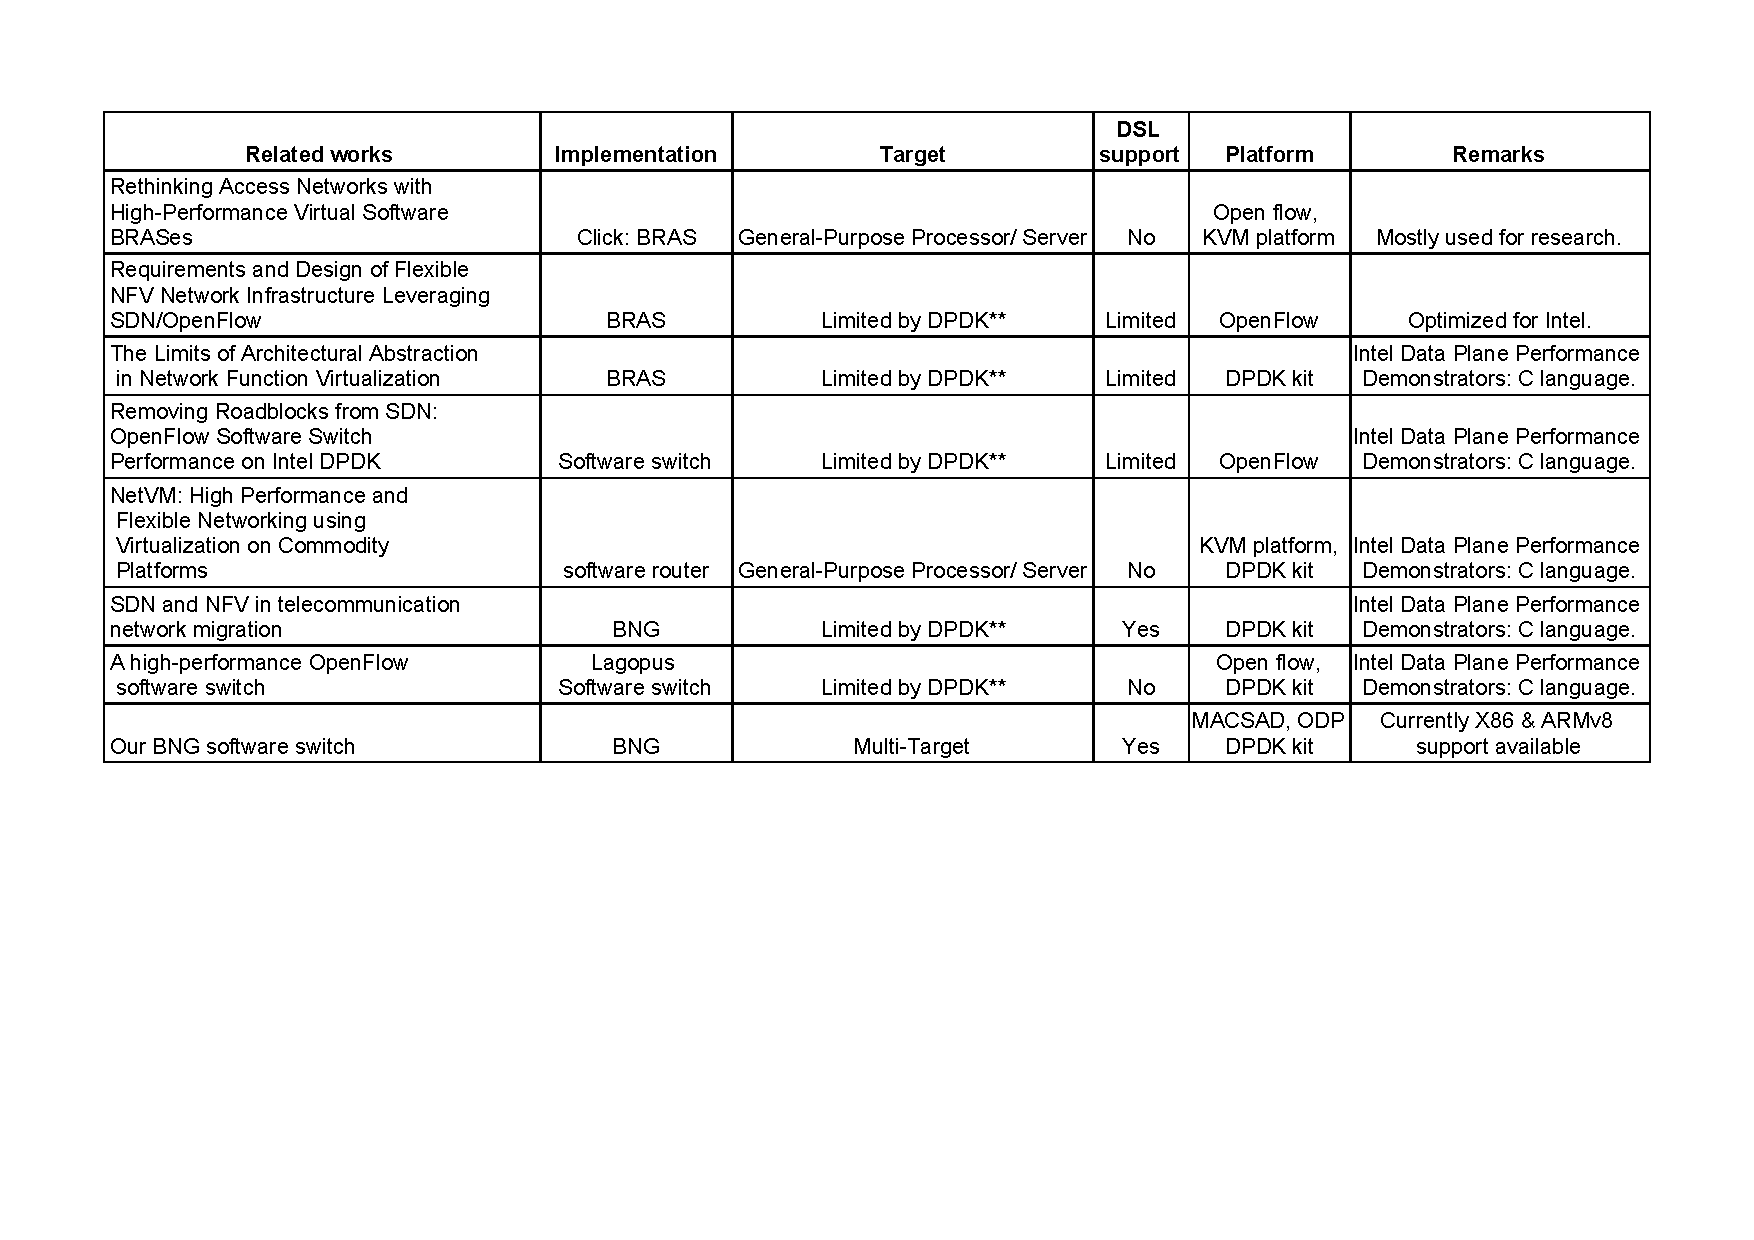
\includegraphics[width=18cm]{figures/related_w.pdf} 
	\end{tabular}
	\caption{Feature comparison list of different Switch software implementations.}
	\label{table:related_w}
\end{table}
